% Name: Scaled dot-product attention
% Description: Queries and keys multiplied, scaled, masked, and normalized, then applied to the values.
% Tags: attention, transformer, softmax

\usetikzlibrary{arrows.meta, positioning}

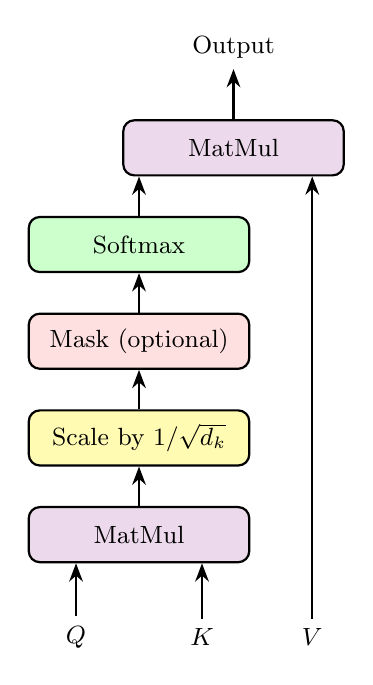
\begin{tikzpicture}[
  node distance=5mm,
  every node/.style={font=\small},
  op/.style={draw, thick, rounded corners, minimum width=28mm, minimum height=7mm},
  arrow/.style={-{Stealth}, thick},
]
  \node[op, fill=violet!15] (mm1) at (0,0) {MatMul};
  \node[op, fill=yellow!30, above=of mm1] (scale) {Scale by $1/\sqrt{d_k}$};
  \node[op, fill=red!12, above=of scale] (mask) {Mask (optional)};
  \node[op, fill=green!20, above=of mask] (soft) {Softmax};
  \node[op, fill=violet!15, above=of soft, xshift=12mm] (mm2) {MatMul};
  \node (q) at (-8mm,-13mm) {$Q$};
  \node (k) at (8mm,-13mm) {$K$};
  \node (v) at (22mm,-13mm) {$V$};

  \draw[arrow] (q) -- (q |- mm1.south);
  \draw[arrow] (k) -- (k |- mm1.south);
  \draw[arrow] (mm1) -- (scale);
  \draw[arrow] (scale) -- (mask);
  \draw[arrow] (mask) -- (soft);
  \draw[arrow] (soft.north) -- (soft.north |- mm2.south);
  \draw[arrow] (v) -- (v |- mm2.south);
  \draw[arrow] (mm2) -- ++(0,10mm) node[above] {Output};
\end{tikzpicture}
